\documentclass[cn]{homework}

\title{作业2}

\begin{document}
    \maketitle    

    \section{题1}
    \begin{subproblem}
        \item
        \begin{figure}[h]
            \centering
            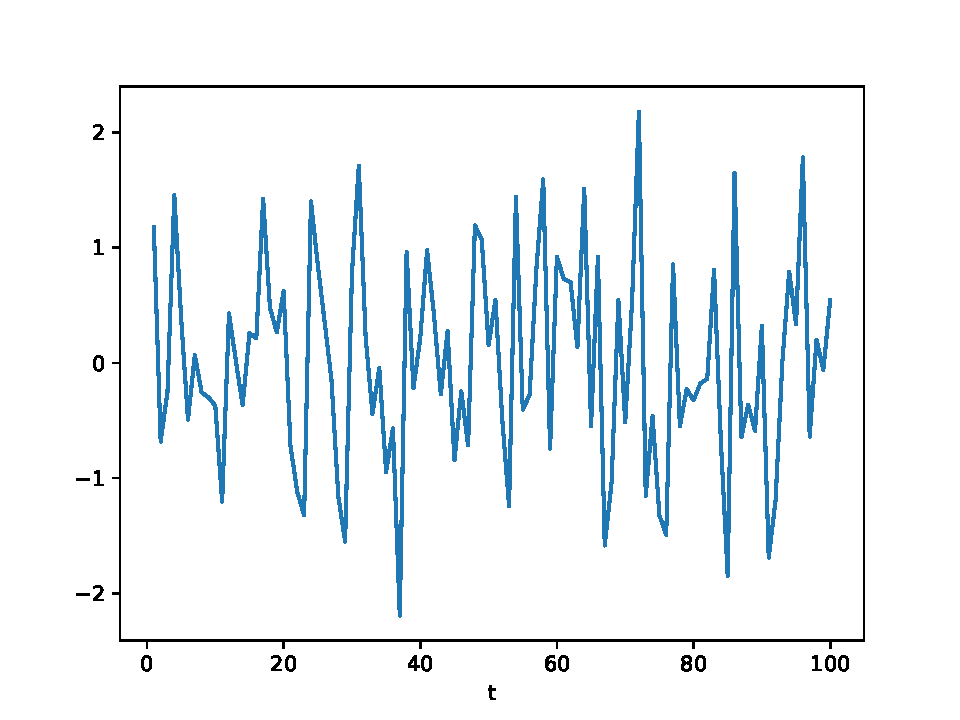
\includegraphics[width=0.45\textwidth]{Xa.pdf}
            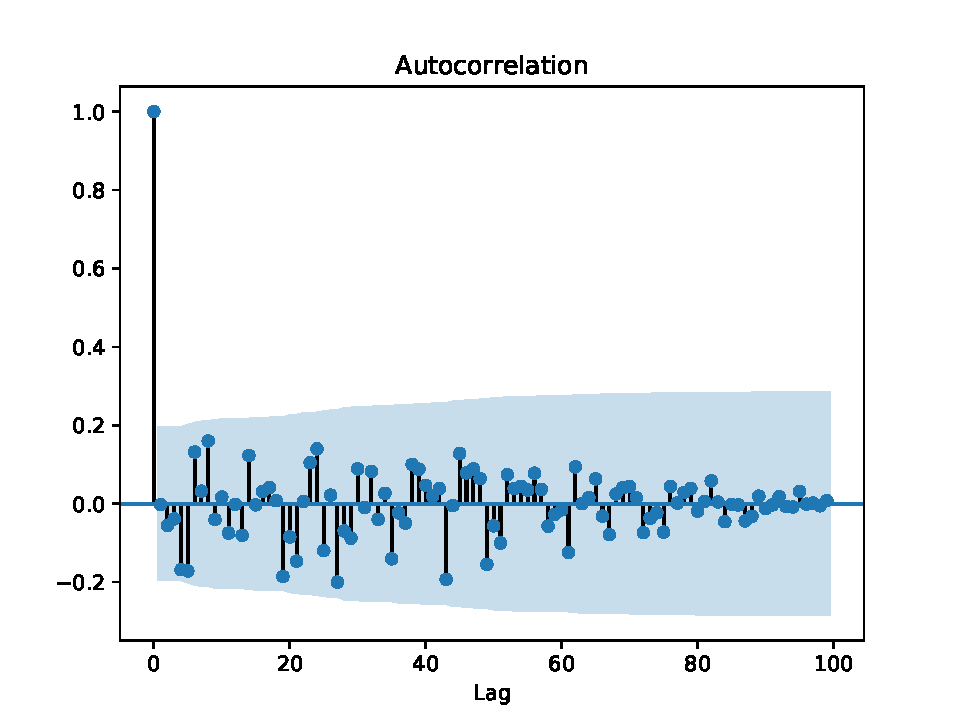
\includegraphics[width=0.45\textwidth]{Xa-acf.pdf}
            \caption{时序图与自相关图:$X_a$}
        \end{figure}

        \item
        \begin{figure}[h]
            \centering
            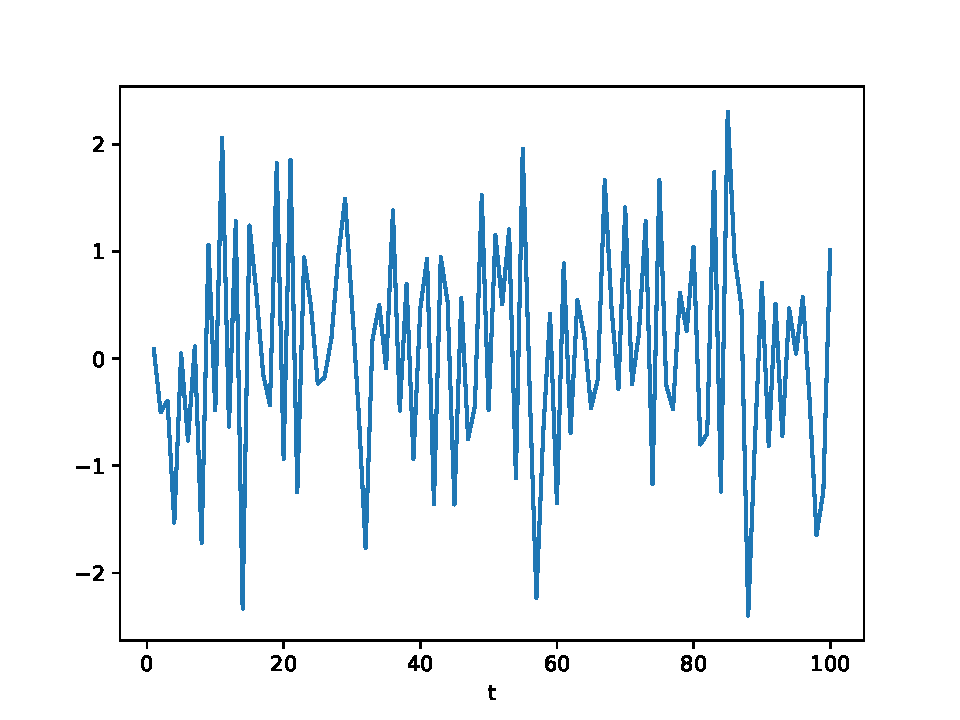
\includegraphics[width=0.45\textwidth]{Xb.pdf}
            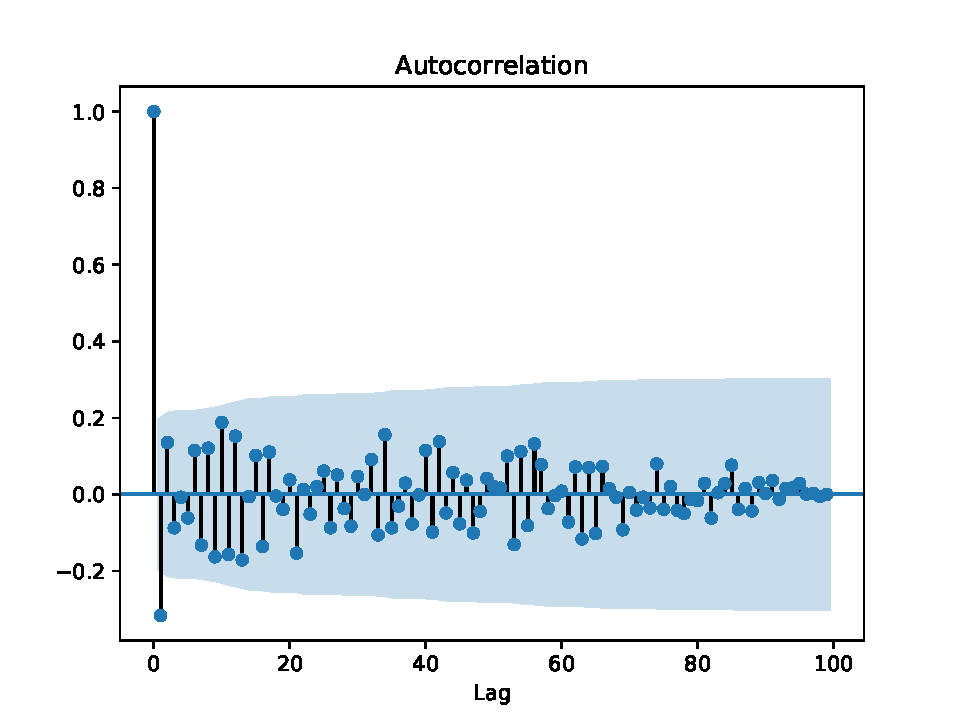
\includegraphics[width=0.45\textwidth]{Xb-acf.pdf}
            \caption{时序图与自相关图:$X_b$}
        \end{figure}

        \item
        \begin{figure}[h]
            \centering
            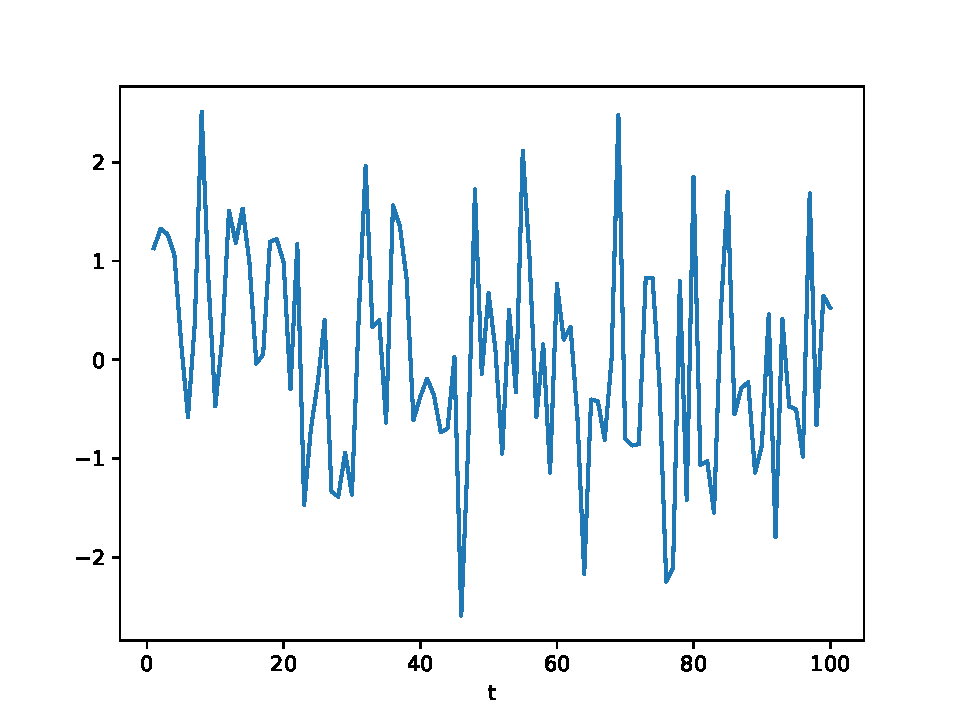
\includegraphics[width=0.45\textwidth]{Xc.pdf}
            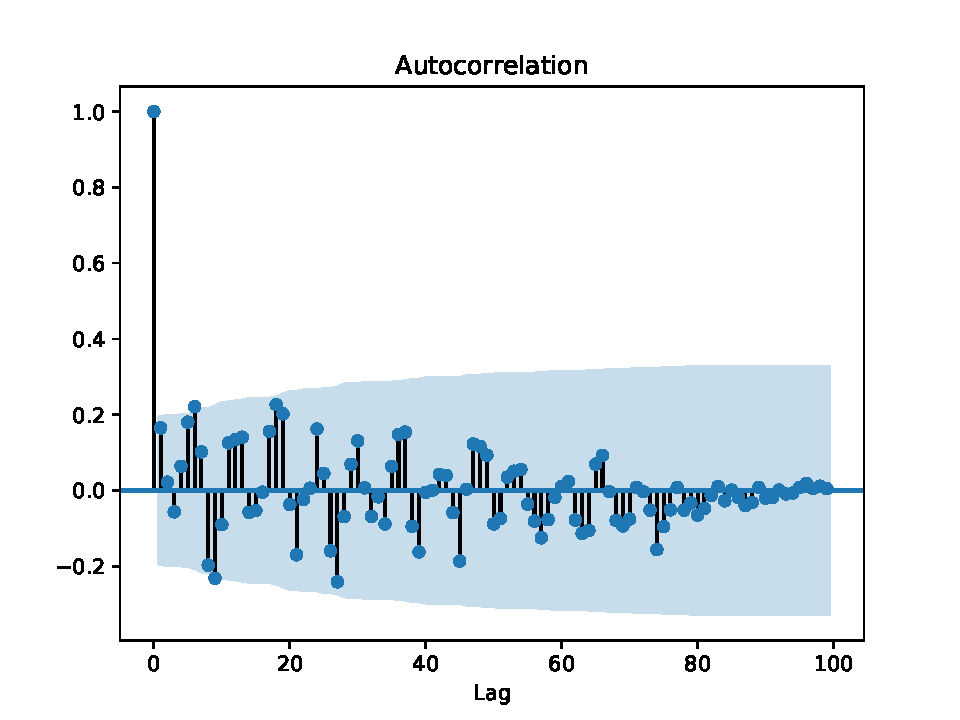
\includegraphics[width=0.45\textwidth]{Xc-acf.pdf}
            \caption{时序图与自相关图:$X_c$}
        \end{figure}

        \item
        \begin{figure}[h]
            \centering
            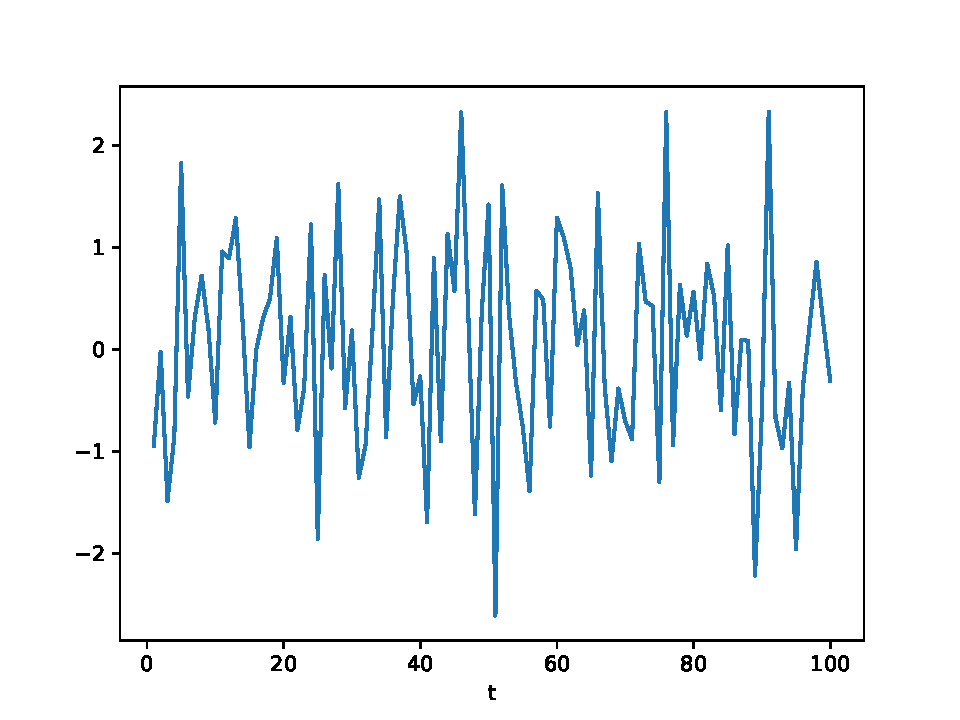
\includegraphics[width=0.45\textwidth]{Xd.pdf}
            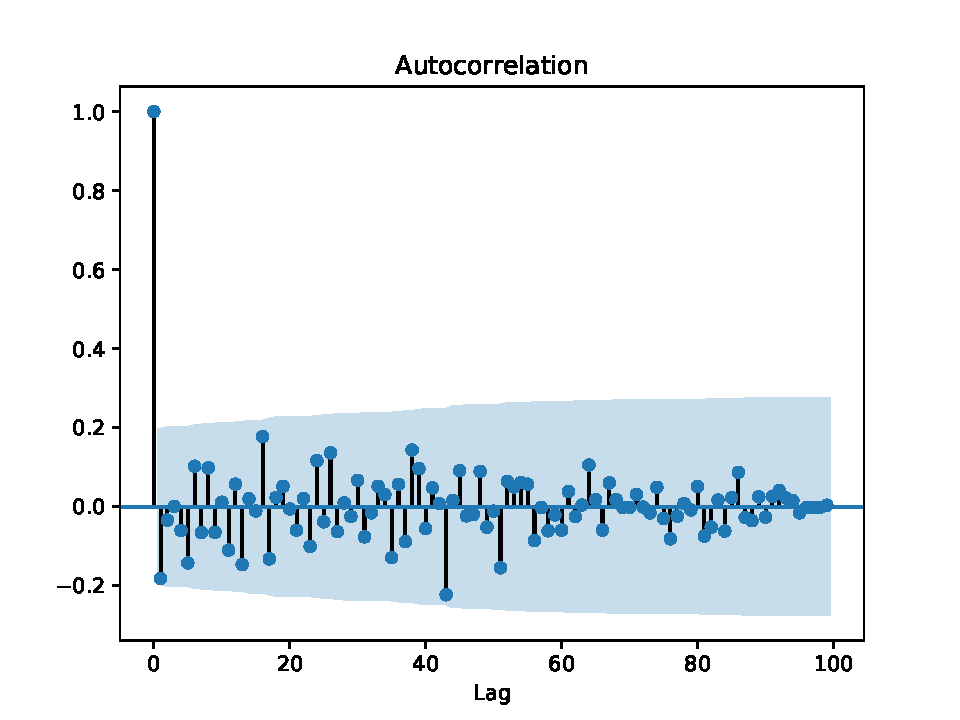
\includegraphics[width=0.45\textwidth]{Xd-acf.pdf}
            \caption{时序图与自相关图:$X_d$}
        \end{figure}

        \item
        \begin{figure}[h]
            \centering
            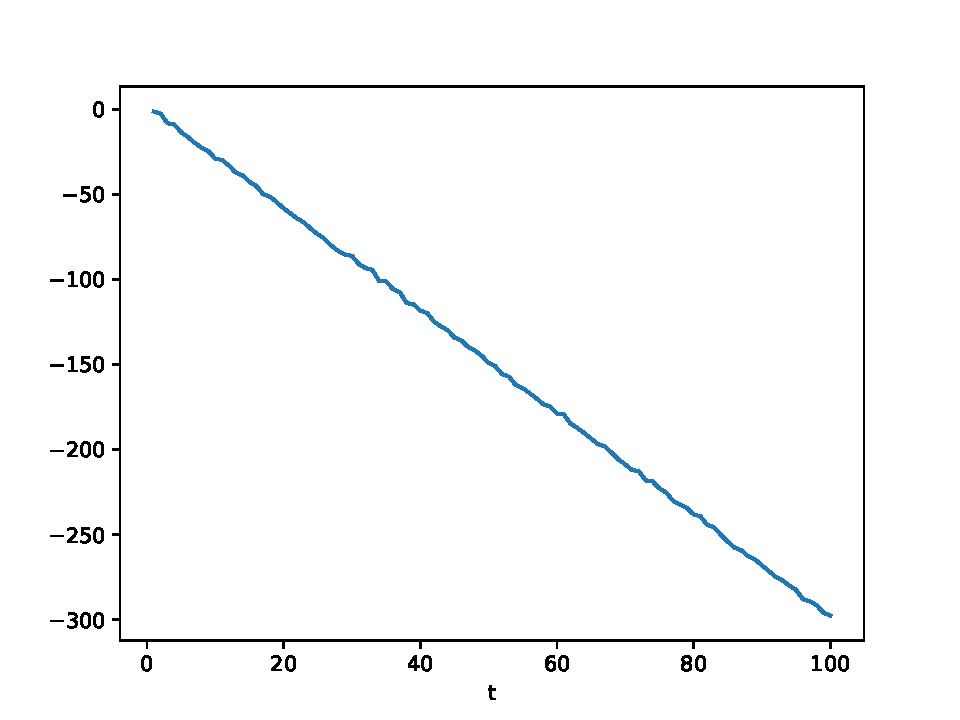
\includegraphics[width=0.45\textwidth]{Xe.pdf}
            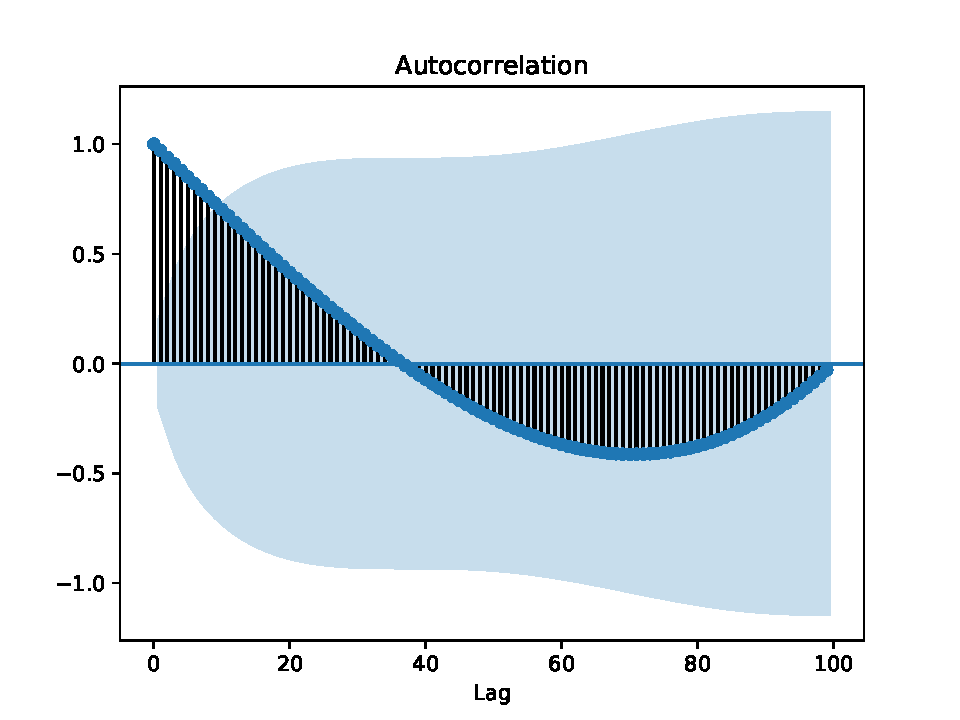
\includegraphics[width=0.45\textwidth]{Xe-acf.pdf}
            \caption{时序图与自相关图:$X_e$}
        \end{figure}
    \end{subproblem}

    \newpage
    \section{题2}
    \begin{subproblem}
        \item
        从时序图上看,观测值在0附近随机波动,同时自相关系数除了开始以外
        始终在2倍标准差内,故应该是一个平稳的时间序列。

        同时分别计算$m=6,12$时的QLB统计量,
        $p$显著大于0.05,因此序列应该是纯随机序列。
        \begin{margintable}
            \begin{tabular}{ccc}
                \toprule
                $m$ & $Q_{\mathrm{LB}}$ & $p$ \\
                \midrule
                6& 8.5377 & 0.2012\\
                12& 12.3465& 0.4182\\
                \bottomrule
            \end{tabular}
        \end{margintable}


        \item
        观测值在0附近波动,也没有明显的周期性,同时自相关系数除了开始
        始终在2倍标准差以内,故应该具有平稳性。

        $p$值显著小于0.05,因此可以拒绝序列是纯随机序列的假设
        \begin{margintable}
            \begin{tabular}{ccc}
                \toprule
                $m$ & $Q_{\mathrm{LB}}$ & $p$ \\
                \midrule
                6 & 14.8603 & 0.0214\\
                12 & 30.8781 & 0.0021\\
                \bottomrule
            \end{tabular}
        \end{margintable}


        \item
        观测值在0附近波动,但是具有一定的周期性,不过自相关系数仍然
        满足平稳时间序列的性质,故应该是平稳的。

        Q统计量的$p$值在$m=6$时不是很显著,在$m=12$时显著小于0.05,
        因此可以拒绝序列是纯随机序列的假设。
        \begin{margintable}
            \begin{tabular}{ccc}
                \toprule
                $m$ & $Q_{\mathrm{LB}}$ & $p$ \\
                \midrule
                6 & 12.4192 & 0.0532\\
                12 & 28.7241 & 0.0043\\
                \bottomrule
            \end{tabular}
        \end{margintable}

        \item
        序列值在0附近波动,也没有很明显的周期性,同时自相关系数也满足
        平稳时间序列的特征,故应该是平稳的。

        Q统计量$p$值显著大于0.05,因此序列应该是纯随机序列。
        \begin{margintable}
            \begin{tabular}{ccc}
                \toprule
                $m$ & $Q_{\mathrm{LB}}$ & $p$ \\
                \midrule
                6 & 7.2507 & 0.2983\\
                12 & 11.0480 & 0.5248\\
                \bottomrule
            \end{tabular}
        \end{margintable}
       

        \item
        时序图和自相关图都明显地与平稳时间序列不符,整体有
        下降趋势,同时自相关系数在一定时间内都很大,故不是平稳的。

        既然不是平稳的,也就不可能是纯随机的,因此也没有纯随机性
        检验的必要。

    \end{subproblem}

    \appendix
    \section{Python代码}
    \lstinputlisting[language=Python,xleftmargin=0pt, xrightmargin=0pt]{ar1.py}
\end{document}